%%%%%%%%%%%%%%%%%%%%%%%%%%%%%%%%%%%%%%%%%%%%%%%%%%%%%%%%%%%%%%%%%%%%%%%%%%
%% CV-SerafinVelezVarrera 0.1, 2014-10-17				%%
%% Written by Serafín Vélez Barrera <serafa12000@gmail.com> 		%%
%% ---------------------------------------------------------- 		%%
%% Licensed under							%%
%% 	Creative Commons Attribution-NonCommercial-ShareAlike 3.0	%%
%% http://creativecommons.org/licenses/by-nc-sa/3.0/			%%
%%%%%%%%%%%%%%%%%%%%%%%%%%%%%%%%%%%%%%%%%%%%%%%%%%%%%%%%%%%%%%%%%%%%%%%%%%

%%%%%%%%%%%%%%%%%%%%%%%%%%%%%%%%%%%%%%%%%%%%%%%%%%%%%%%%%%%%%%%%%%%%%%%%%%
%				Preámbulo				 %
%%%%%%%%%%%%%%%%%%%%%%%%%%%%%%%%%%%%%%%%%%%%%%%%%%%%%%%%%%%%%%%%%%%%%%%%%%


% Definición del documento
\documentclass{beamer}
\usepackage[utf8x]{inputenc}
\usepackage[spanish]{babel}
\usepackage{beamerthemeshadow}
\usepackage{hyperref}
\usepackage{ragged2e} 
\usetheme{Antibes}


% Preámbulo -> Definición del título del documento, autor, institución, fecha y fondo para las transparencias.
\title{GtkRecordMyDesktop}
\subtitle{A grabar se ha dicho}
\author[Serafín Vélez Barrera]{Serafín Vélez Barrera\\ \scriptsize{\texttt{\href{mailto:serafa12000@gmail.com}{serafa12000@gmail.com}} -- \href{http://twiter.com/seravb}{@seravb}}}
\date{3/12/12}
%\institute{
\includegraphics[scale=0.5]{Imagenes/LogoOSL.png} \\ \flushright 
\includegraphics[scale=0.5, keepaspectratio=true]{Licencia/By-sa.png}}
\institute{\href{http://osl.ugr.es}{
\includegraphics[scale=0.5]{Imagenes/LogoOSL.png}} \\ \flushright \href{http://creativecommons.org/licenses/by-sa/3.0/deed.es_ES}{
\includegraphics[scale=0.5, keepaspectratio=true]{Licencia/By-sa.png}}}
\usebackgroundtemplate{
\includegraphics[width=\textwidth]{Imagenes/GTK-RecordMyDesktop2.png}}



% Comandos personalizados
\newcommand{\negrita} % Texto en negrita
[1]{\textbf{#1}}
\newcommand{\cursiva} % Texto en cursiva
[1]{\textit{#1}}
\newcommand{\negritacursiva} % Texto en negrita-cursiva
[1]{\textbf{\textit{#1}}}


% Documento
\begin{document}
	\begin{frame}
		\titlepage
	\end{frame}


	\begin{frame}
	        \frametitle{Índice}
	        \tableofcontents
	\end{frame}


	\section{Introducción}
% 		\begin{frame}
% 			\frametitle{¿Quién soy?}
% 			\Huge ¿Quién soy?
% 			\normalsize Técnico de la OSL e Ing. Téc. Informática
% 		\end{frame}
% 		\begin{frame}
% 			\frametitle{Programo}
% 			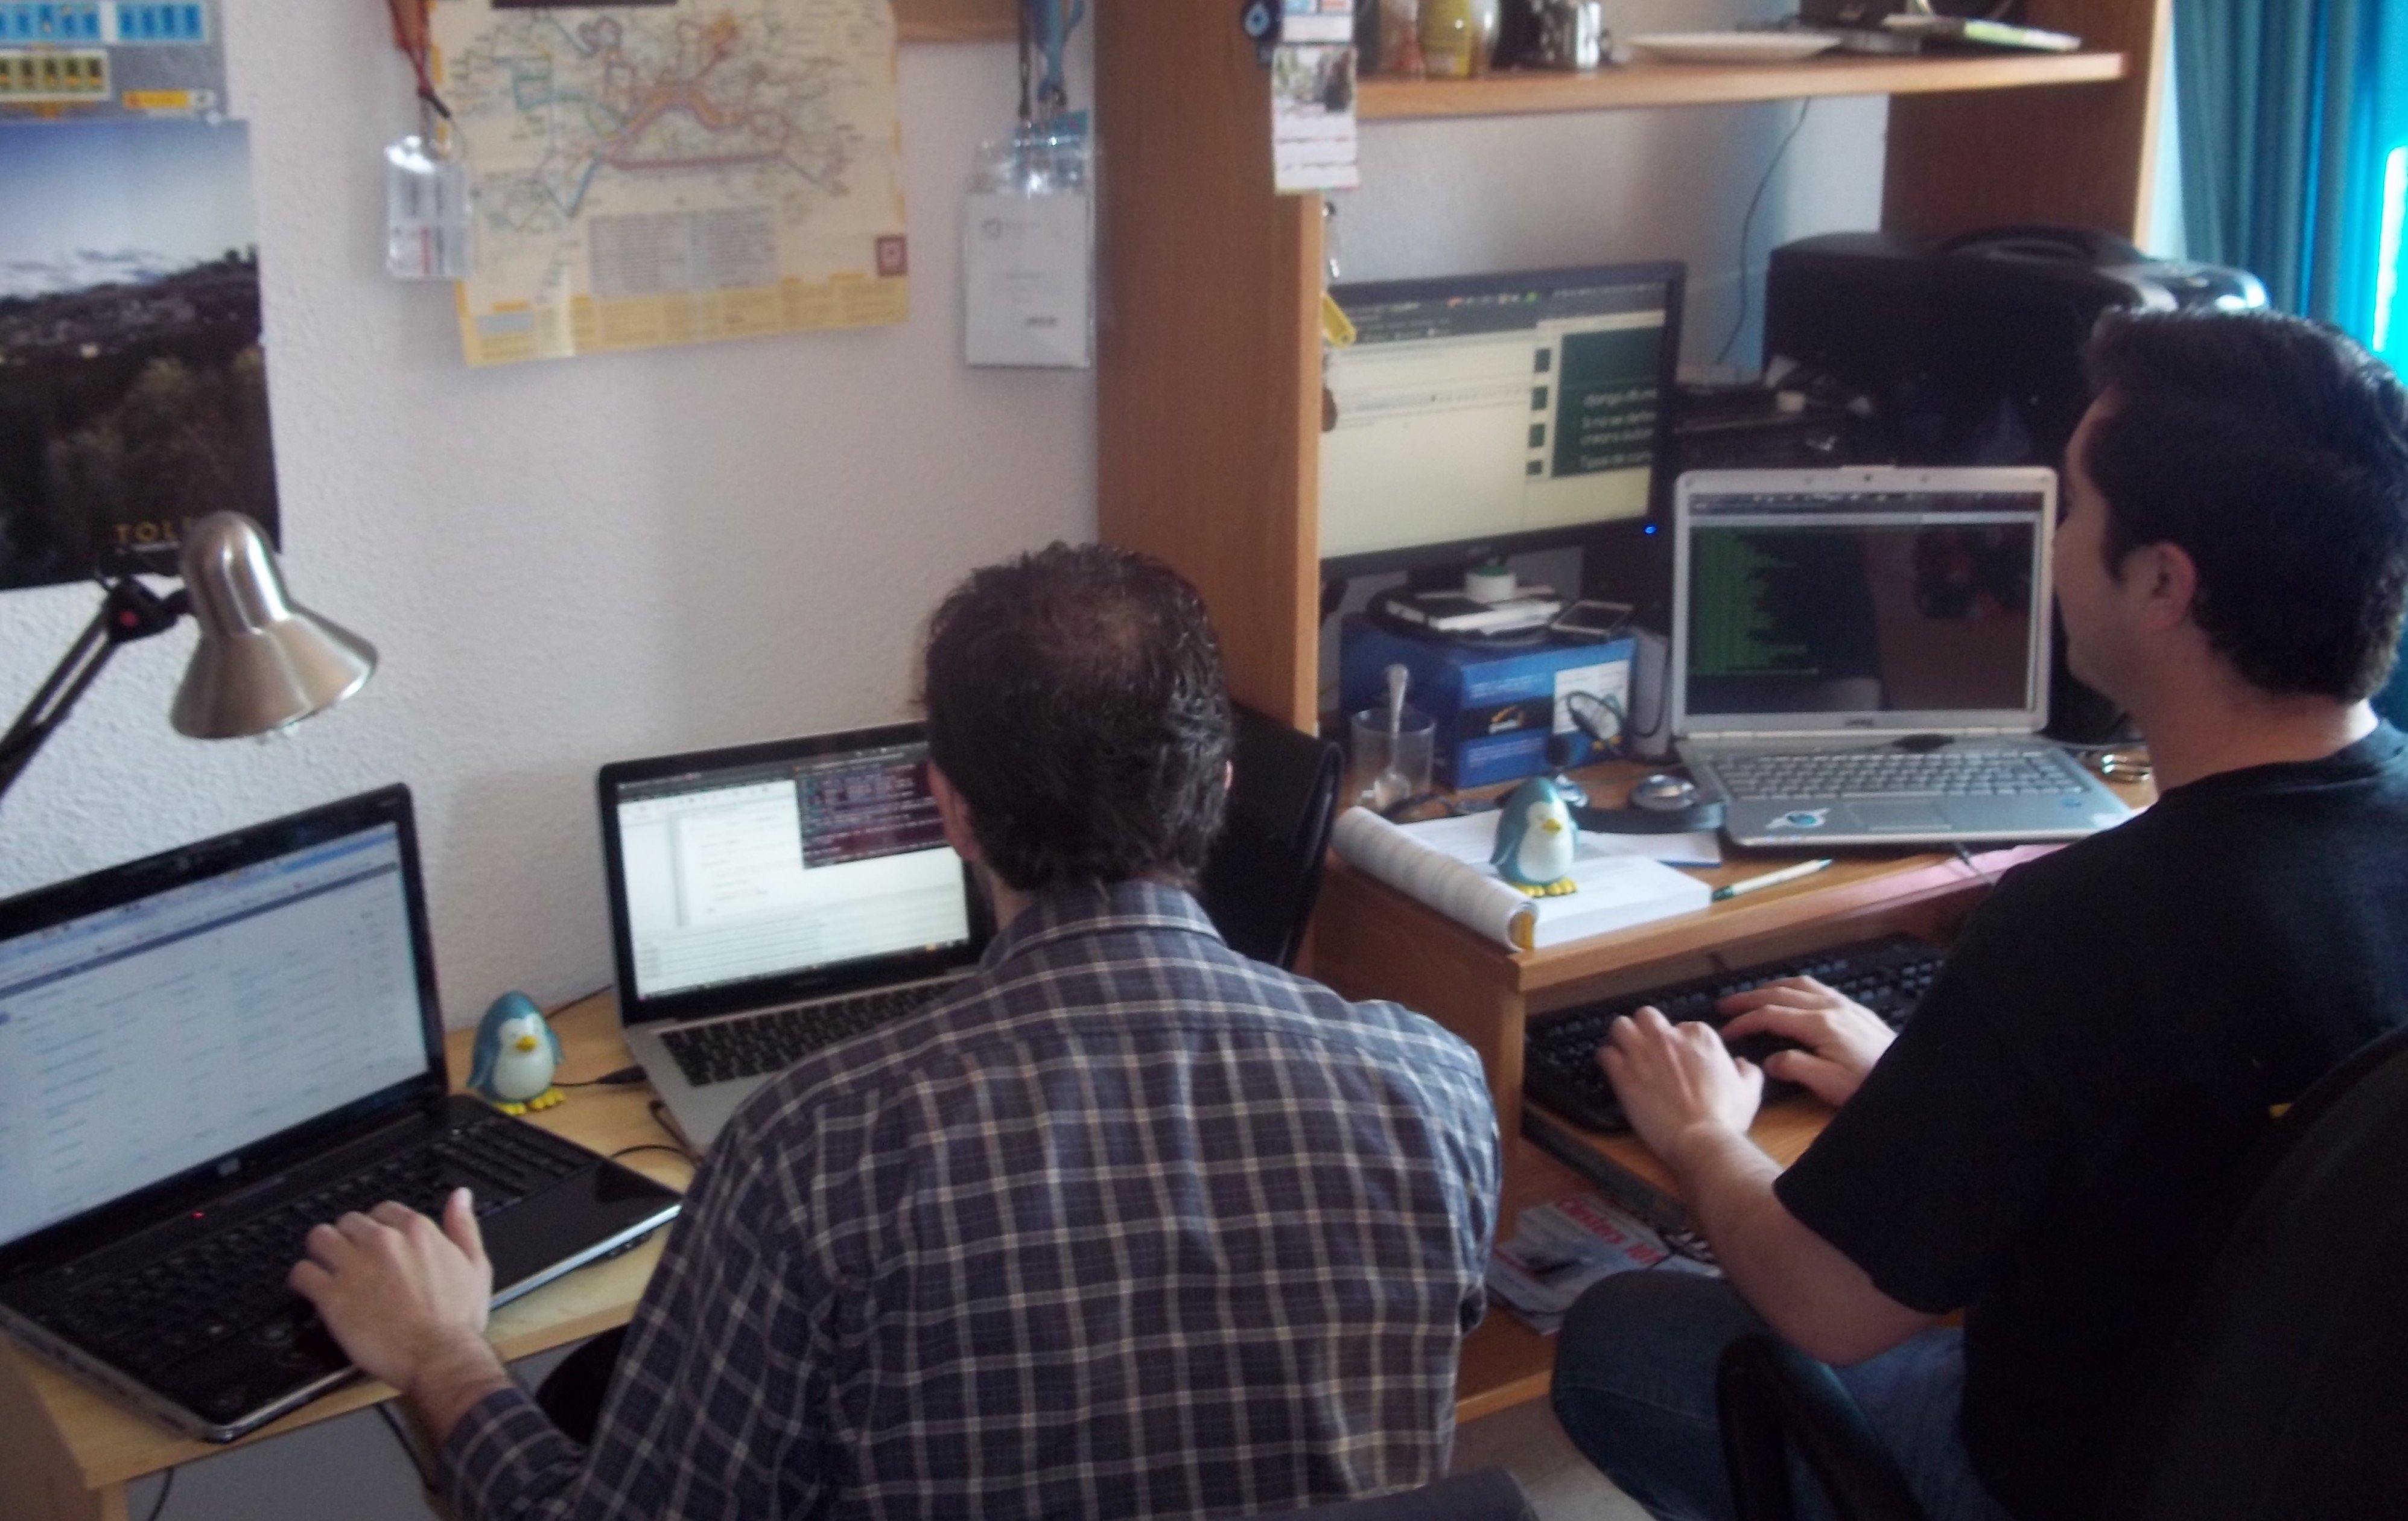
\includegraphics[width=\textwidth, keepaspectratio=true]{Imagenes/Fotos/Programando.jpg}
% 		\end{frame}
% 		\begin{frame}
% 			\frametitle{Reciclo equipos}
% 			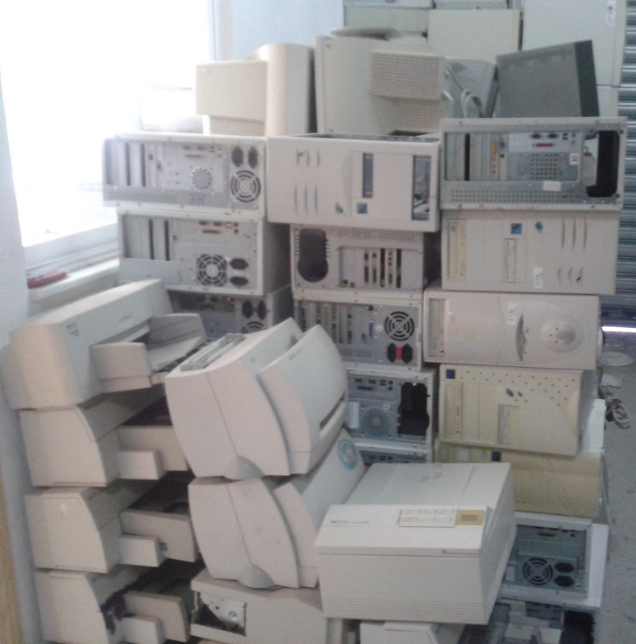
\includegraphics[height=\textheight, keepaspectratio=true]{Imagenes/Fotos/Reciclando.png}
% 		\end{frame}
% 		\begin{frame}
% 			\frametitle{Cocino tuxes}
% 			\begin{center}
% 				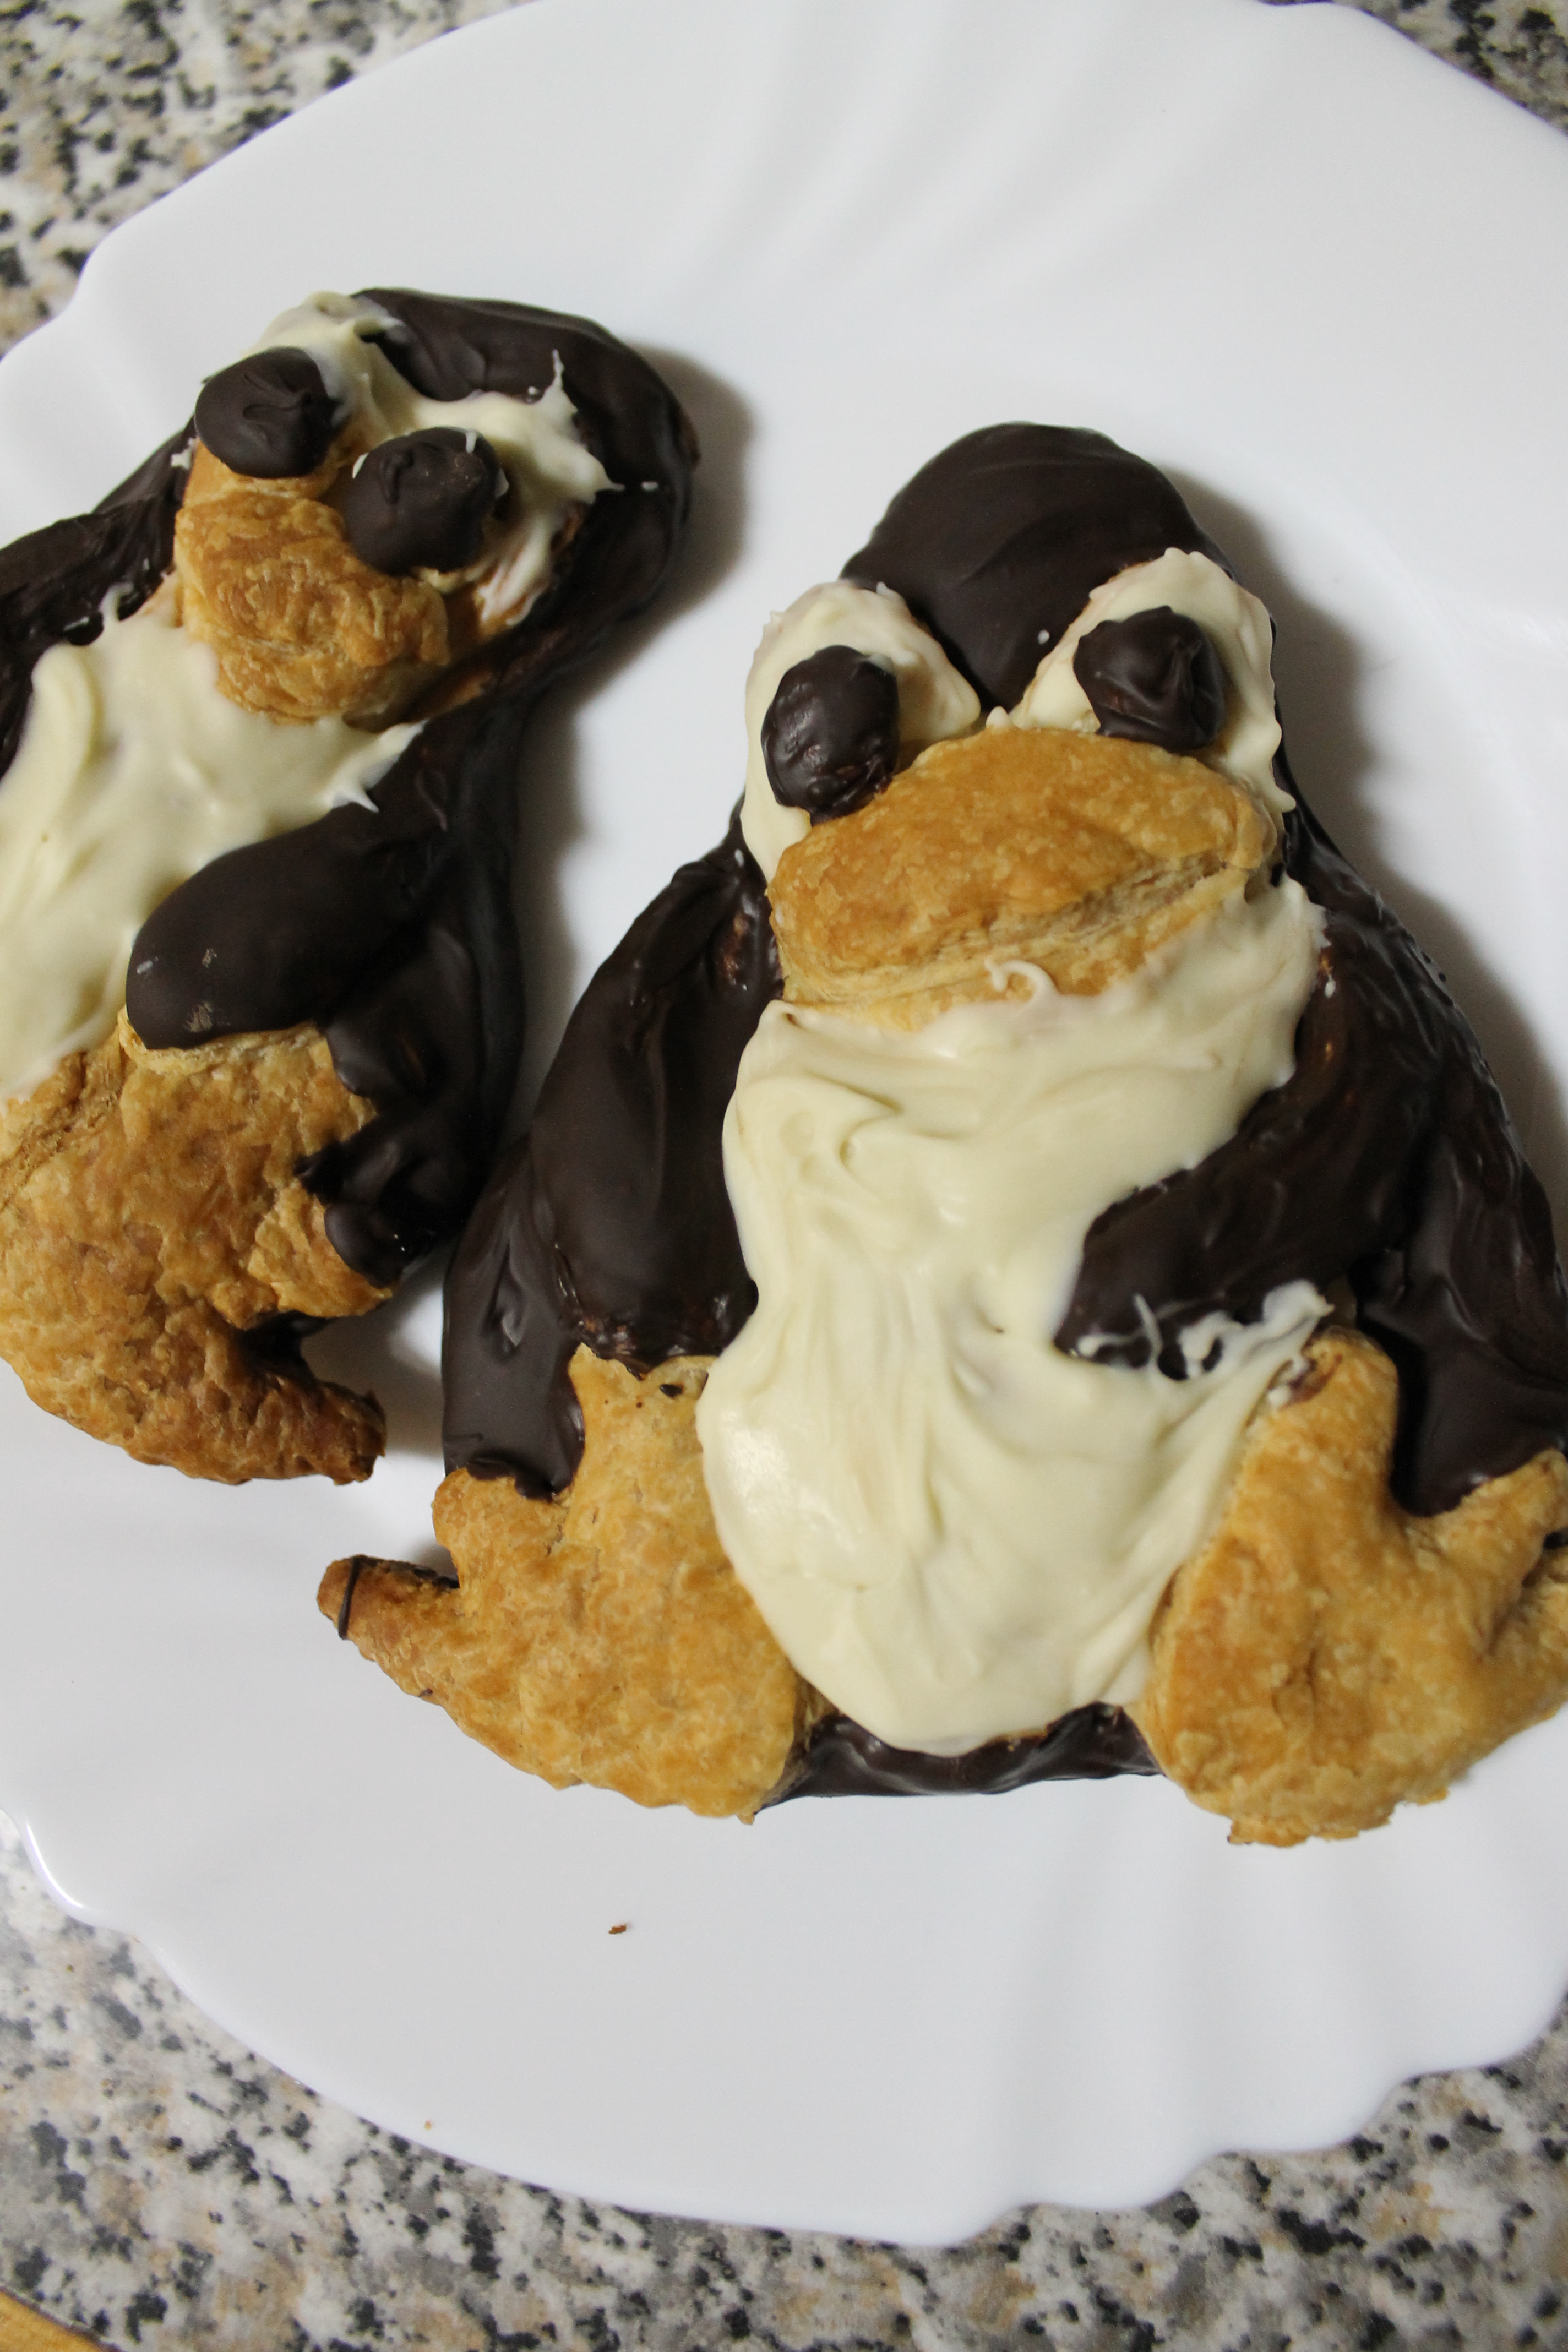
\includegraphics[height=\textheight, keepaspectratio=true]{Imagenes/Fotos/Cocinando.JPG}
% 			\end{center}
% 		\end{frame}
% 		\begin{frame}
% 			\frametitle{Hago cubiletes}
% 			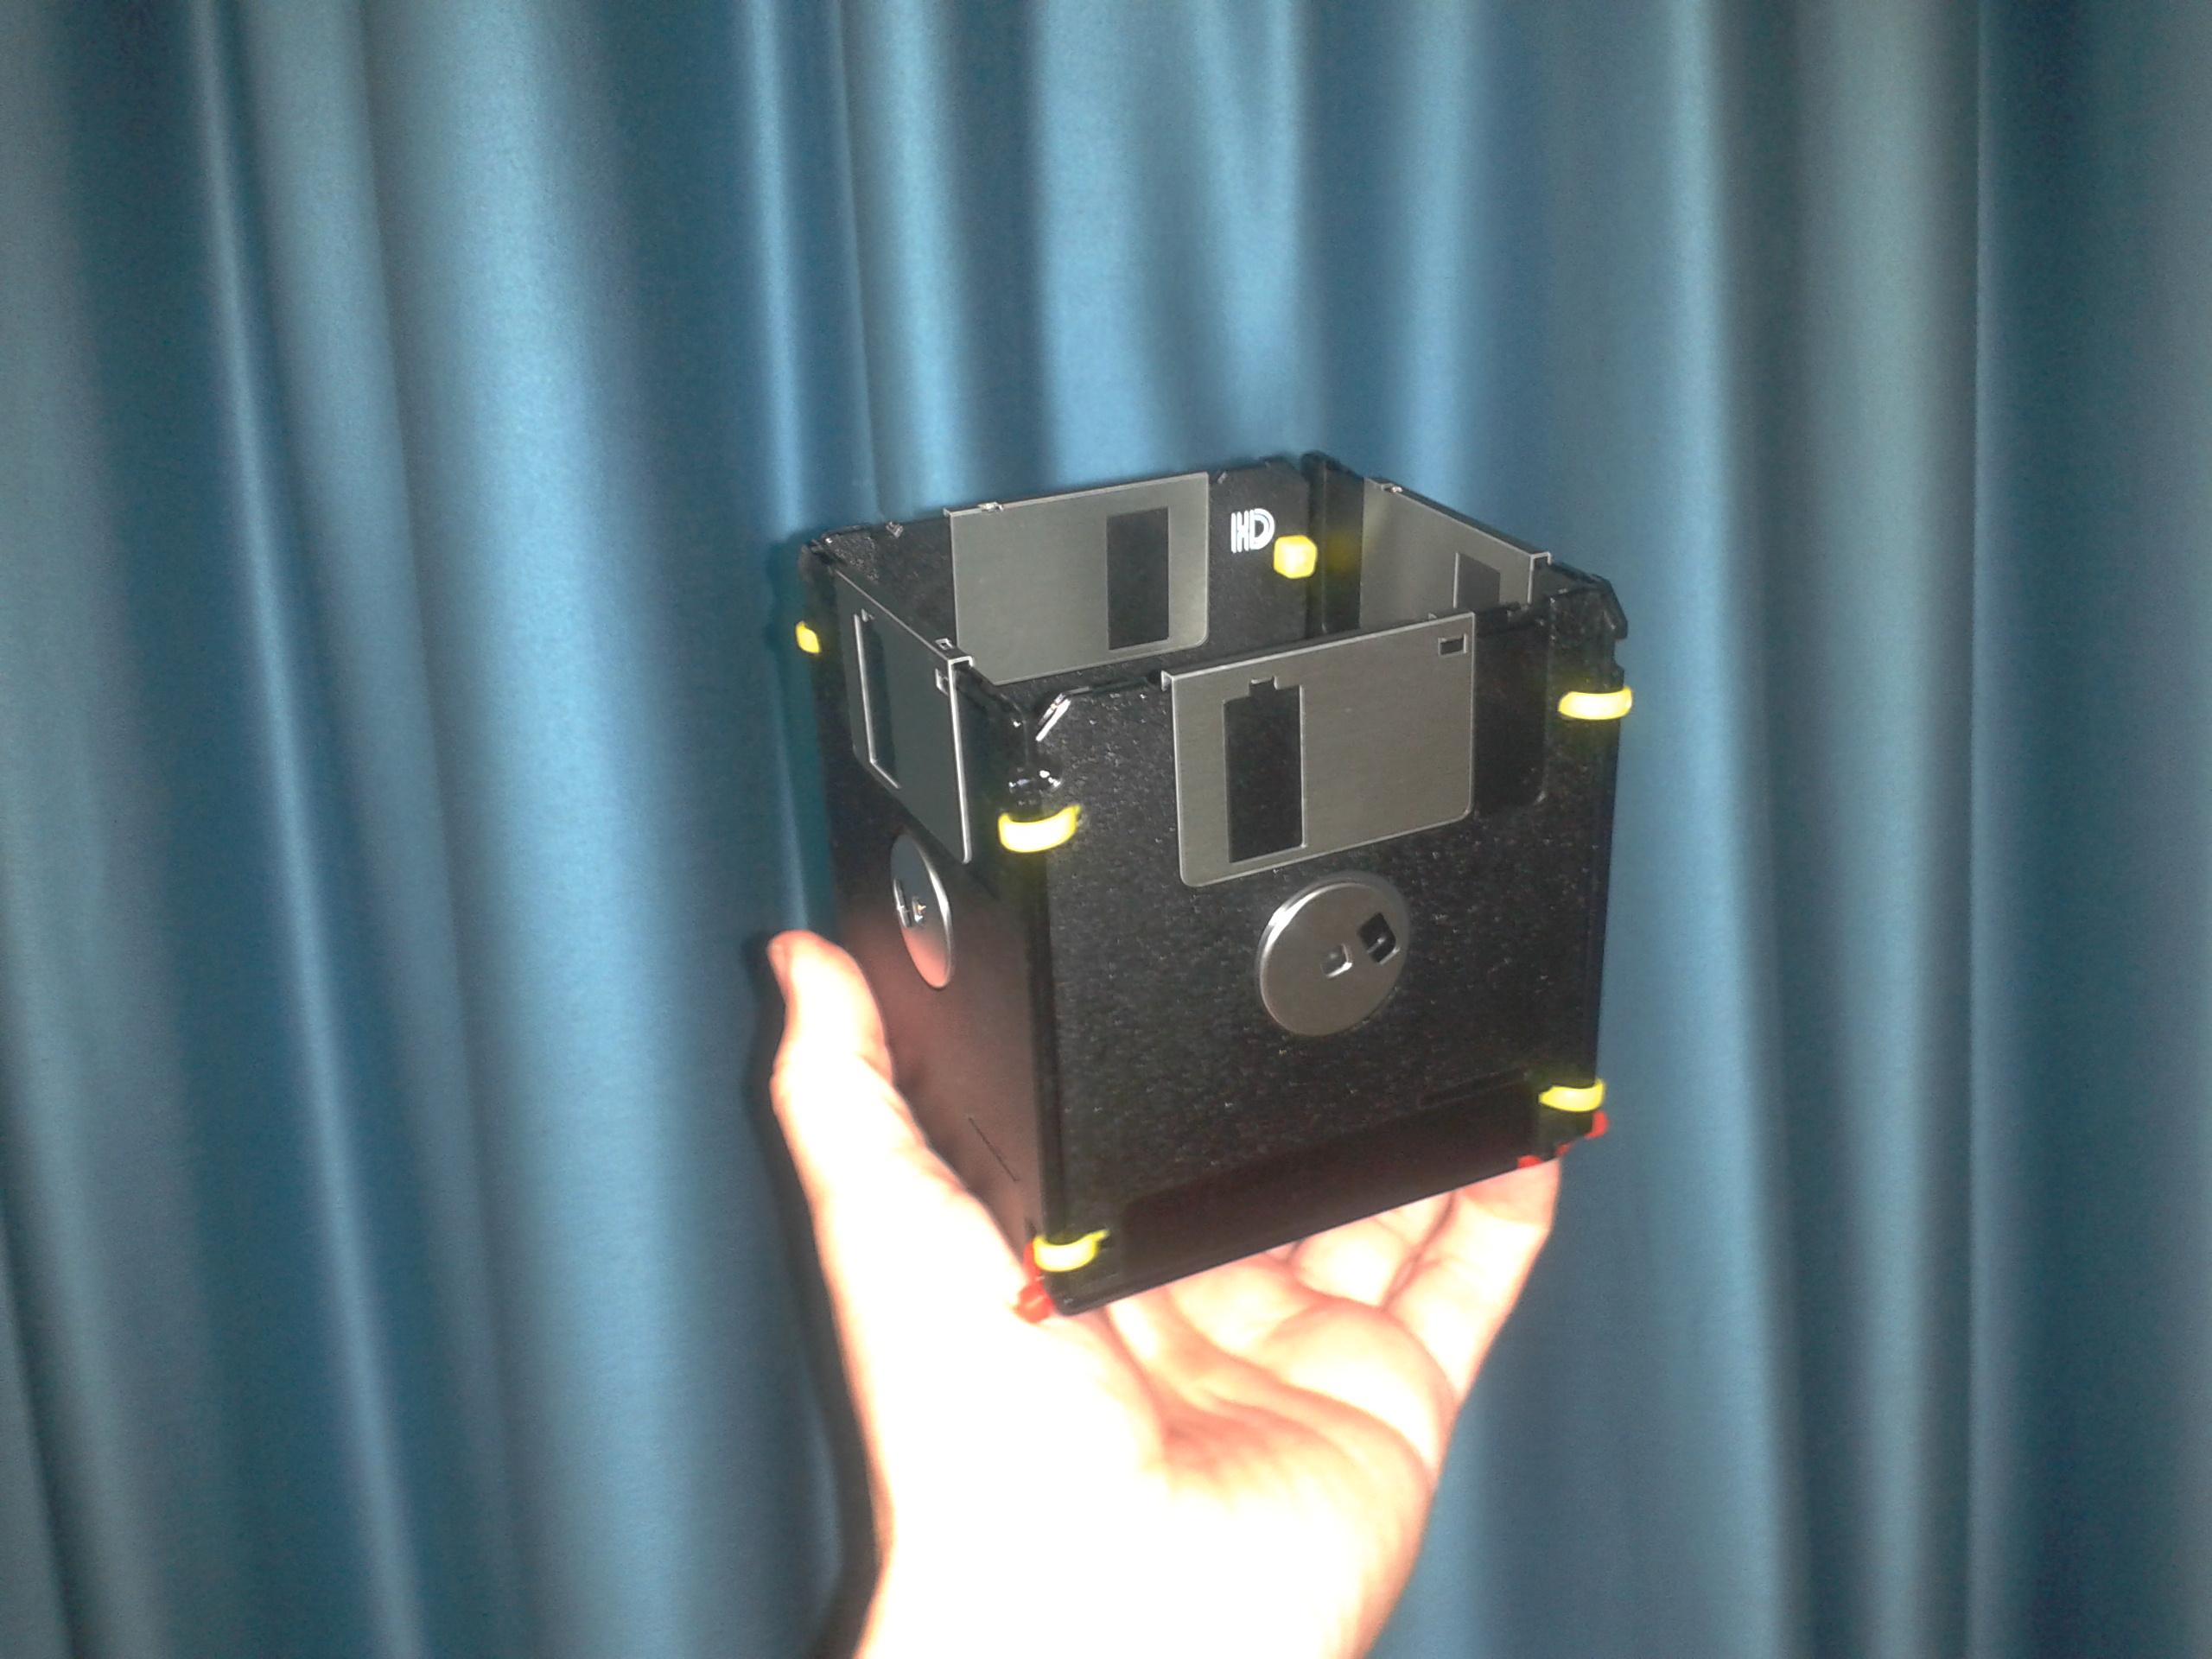
\includegraphics[height=\textheight, keepaspectratio=true]{Imagenes/Fotos/Cubilete.jpg}
% 		\end{frame}
		\begin{frame}
			\frametitle{Aplicaciones multimedia}
			\begin{itemize}
				\item Edición de audio: Grabadora de sonido, \negrita{Audacity}, etc.
				\item Edición de vídeo: Pitivi, Openshot, \negrita{Kdenlive}, etc.
				\item Edición de imágen: \negrita{Gimp}, \negrita{Inkscape}, Tuxpaint, etc
				\item Escritorio: Istanbul, Wink, \negrita{GtkRecordMyDesktop}, \cursiva{Camtasia}, etc
				\item Varios: Reproductores, webcams, subtítulos, etc
			\end{itemize}
		\end{frame}
		\begin{frame}
			\frametitle{¿Entonces qué es GtkRecordMyDesktop?}
			\large Es un programa para grabar vídeos y audio sobre lo que está ocurriendo en el escritorio.
			\begin{flushleft}
				\Large{¿Para que me sirve?}
			\end{flushleft}
				\pause
			\begin{flushright}
				\LARGE{Para hacer demostraciones, tutoriales y screencasts}.
			\end{flushright}
		\end{frame}


	\section{Instalación}
		\begin{frame}
			\frametitle{Instalación}
			Podremos instalar GTK-RecordMyDesktop bien desde el centro de software o algún gestor de paquetes:
			\begin{center}
				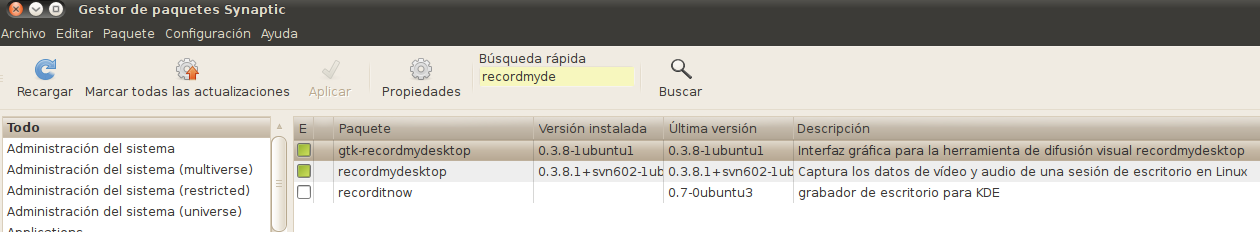
\includegraphics[height=0.3\textheight, keepaspectratio=true]{Imagenes/Instalacion/01_Synaptic.png}
			\end{center}
			O bien desde la terminal:
			\begin{center}
				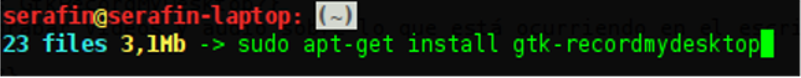
\includegraphics[height=0.1\textheight, keepaspectratio=true]{Imagenes/Instalacion/02_Terminal.png}
			\end{center}
		\end{frame}


	\section{Hoja de ruta}
		\begin{frame}
			\frametitle{Hoja de ruta- I}
			\justifying 
			Sigue estos pasos para crear tu videotutorial o screencast:
			\begin{itemize}
				\item <1-> Piensa que quieres hacer.
				\item <2-> Empieza por hacerte un guión con una tabla de tiempos. 
				\item <3-> Configura el sistema operativo si es necesario (desactiva los efectos visuales, decoración de ventanas, etc).
				\item <4-> Configura el programa según tus gustos y según tus necesidades (ruta de almacenamiento de vídeos, canales de sonido).
			\end{itemize}
		\end{frame}
		\begin{frame}
			\frametitle{Hoja de ruta - II}
			\justifying 
			Sigue estos pasos para crear tu videotutorial o screencast:
			\begin{itemize}
				\item <1-> Con el guión que te has hecho graba los vídeos.
				\item <2-> Separa el audio del vídeo para procesarlo si es necesario.
				\item <3-> Monta el vídeo final con los vídeos que has grabado.
				\item <4-> Cambia el formato del vídeo de OGV a AVI, MP4, etc.
				\item <5-> Publícalo en internet, en tu exposición de clase, etc.
			\end{itemize}
		\end{frame}
		\begin{frame}
			\frametitle{Hoja de ruta - III}
			\justifying 
			\Huge{Notas}
			\normalsize
			\begin{itemize}
				\item Usa boli y papel si es necesario.
				\item Usa una hoja de cálculo.
				\item Sigue el orden de tu guión.
				\item No olvides hacer los recortes pertinentes.
				\item Indica los medios para contactar contigo (email, twitter, etc).
			\end{itemize}
		\end{frame}


	\section{Interfaz}
		\begin{frame}
			\frametitle{Interfaz}
			\begin{columns}
				\begin{column}[l]{5cm}
					La ventana principal:
					\begin{enumerate}
						\item Área de previsualización
						\item Botones de grabación
						\item Controles de vídeo y audio
					\end{enumerate}
				\end{column}
				\begin{column}[r]{5cm}
					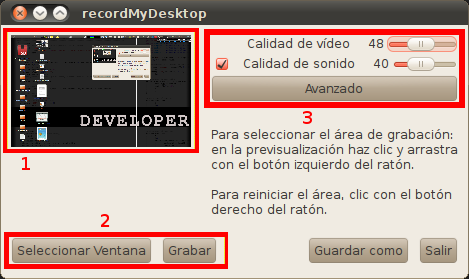
\includegraphics[height=0.4\textheight, keepaspectratio=true]{Imagenes/Interfaz/01.png}
				\end{column}
			\end{columns}
		\end{frame}
		\begin{frame}	
			\frametitle{Configuración del programa(I) - Archivos}
			\begin{columns}
				\begin{column}[l]{5cm}
					\justifying 
					En las opciones avanzadas encontramos aquí el lugar para guardar los vídeos y si los queremos sobreescribir si existieran ya.
				\end{column}
				\begin{column}[r]{5cm}
					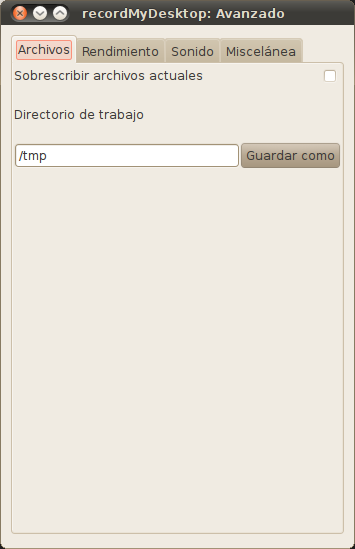
\includegraphics[height=0.8\textheight, keepaspectratio=true]{Imagenes/Interfaz/02.png}
				\end{column}
			\end{columns}
		\end{frame}
		\begin{frame}
			\frametitle{Configuración del programa(II) - Rendimiento}
			\begin{columns}
				\begin{column}[l]{6cm}
					\justifying 
					\begin{enumerate}
						\item Imágenes por segundo -- A más imágenes vídeo de mayor fluidez
						\item Codificación al vuelo - Mayor uso del procesador
						\item Compresión del vídeo -- Sin compresión el vídeo es más pesado
						\item Submuestreo rápido de la imagen -- Menor uso del procesador 
					\end{enumerate}
				\end{column}
				\begin{column}[r]{4cm}
					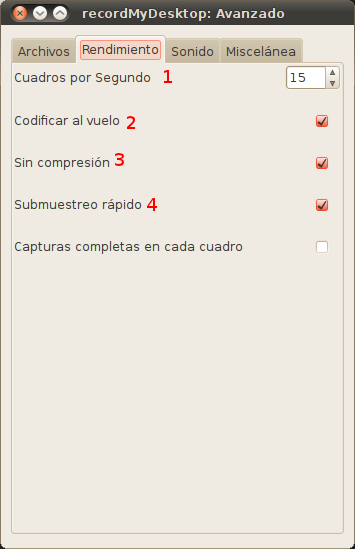
\includegraphics[height=0.8\textheight, keepaspectratio=true]{Imagenes/Interfaz/03.png}
				\end{column}
			\end{columns}
		\end{frame}
		\begin{frame}
			\frametitle{Configuración del programa(III) - Sonido}
			\begin{columns}
				\begin{column}[l]{5cm}
					\justifying
					\begin{enumerate}
						\item Número de canales de sonido
						\item Frecuencia de muestreo
						\item Dispositivo de captura
						\item Selección de fuente de sonido (usar jack)
					\end{enumerate}
				\end{column}
				\begin{column}[r]{5cm}
					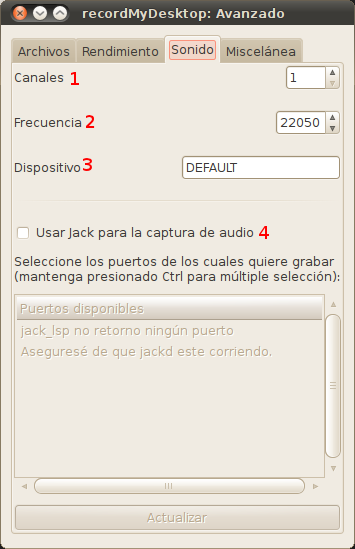
\includegraphics[height=0.8\textheight, keepaspectratio=true]{Imagenes/Interfaz/04.png}
				\end{column}
			\end{columns}
		\end{frame}
		\begin{frame}
			\frametitle{Configuración del programa(IV) - Miscelánea}
			\begin{columns}
				\begin{column}[l]{5cm}
					\justifying
					\begin{enumerate}
						\item Tipo de cursor para el ratón
						\item Habilitar el seguimiento del ratón por el escritorio
						\item Al seleccionar las ventanas incluir la barra de título
						\item Habilitar la ayuda del programa
						\item Dibujar un marco de la selección de la zona a grabar
						\item Configuración más avanzada: Display, extensión MIT-Shm...
					\end{enumerate}
				\end{column}
				\begin{column}[r]{5cm}
					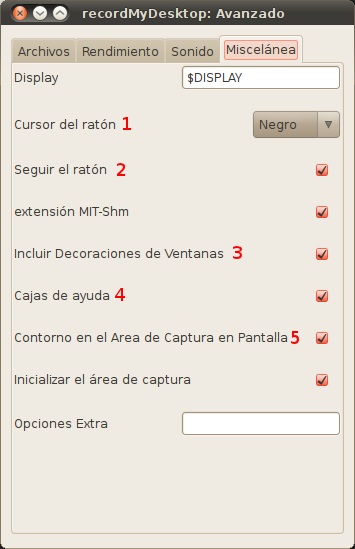
\includegraphics[height=0.8\textheight, keepaspectratio=true]{Imagenes/Interfaz/05.png}
				\end{column}
			\end{columns}
		\end{frame}
		\begin{frame}
			\frametitle{Grabando - I}
			\begin{columns}
				\begin{column}[l]{5cm}
					\justifying
					Botón para empezar la grabación, está en el área de notificación del sistema
				\end{column}
				\begin{column}[r]{5cm}
					
\includegraphics[width=0.9\textwidth, keepaspectratio=true]{Imagenes/Interfaz/06.png}
				\end{column}
			\end{columns}
		\end{frame}
		\begin{frame}
			\frametitle{Grabando - II}
			\begin{columns}
				\begin{column}[l]{5cm}
					\justifying 
					Botón para pausar y/o detener la grabación, está en el área de notificación del sistema
				\end{column}
				\begin{column}[r]{5cm}
					
\includegraphics[width=0.9\textwidth, keepaspectratio=true]{Imagenes/Interfaz/07.png}
				\end{column}
			\end{columns}
		\end{frame}
		\begin{frame}
			\frametitle{Resultados}
			\begin{columns}
				\begin{column}[l]{5cm}
					\justifying 
					Al detener por completo la grabación se procesarán los datos de vídeo y audio para almacenarlos.
				\end{column}
				\begin{column}[r]{5cm}
					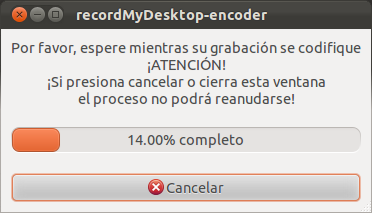
\includegraphics[height=0.4\textheight, keepaspectratio=true]{Imagenes/Interfaz/08.png}
				\end{column}
			\end{columns}
		\end{frame}


	\section{Conclusiones}
		\begin{frame}
			\frametitle{Conclusión}
			\justifying 
			\begin{itemize}
				\item Una vez visto el programa es cuestión de probarlo, probarlo y de nuevo probarlo.
				\item Si no tienes prisa, tómate tu tiempo para grabar y vuelve a grabar si es necesario.
				\item Planifícate bien y todo irá mucho mejor.
			\end{itemize}
		\end{frame}
		\begin{frame}
			\begin{center}
				
\includegraphics[height=\textheight, keepaspectratio=true]{Imagenes/PreguntasDudasAclaraciones.png}
			\end{center}
		\end{frame}
		\begin{frame}
			\begin{center}
				\Huge{\textbf{MUCHAS GRACIAS}}
				¡Y con esto y un bizcocho, el que diga que esto fue difícil miente como Pinocho!
			\end{center}
		\end{frame}

		% BIBLIOGRAFÍA
		\begin{frame}
			\frametitle{Bibliografía}
			\begin{itemize}
				\item \href{http://recordmydesktop.sourceforge.net/about.php}{Web oficial}
				\item \href{http://osl.ugr.es/wp-content/uploads/2012/07/Manual-de-GtkRecordMyDesktop.pdf}{Apuntes del Campus Infantil de Soft. Libre}
			\end{itemize}
		\end{frame}

		% LICENCIA
		\begin{frame}
			\frametitle{Licencia}
			\begin{figure}
				
\includegraphics[keepaspectratio=true]{Licencia/By-sa.png}
			\end{figure}
			\begin{center}
				\Large GTK-RecordMyDesktop by \textbf{\href{http://seravb.wordpress.com}{Serafín Vélez Barrera}} is licensed under a
				\textbf{\href{http://creativecommons.org/licenses/by-sa/3.0/deed.es_ES}{Creative Commons Reconocimiento-CompartirIgual 3.0 Unported License}}.
			\end{center}
		\end{frame}
\end{document}
